\documentclass[tikz]{standalone}

\usepackage{amsmath}

\usetikzlibrary{arrows.meta}

\begin{document}
    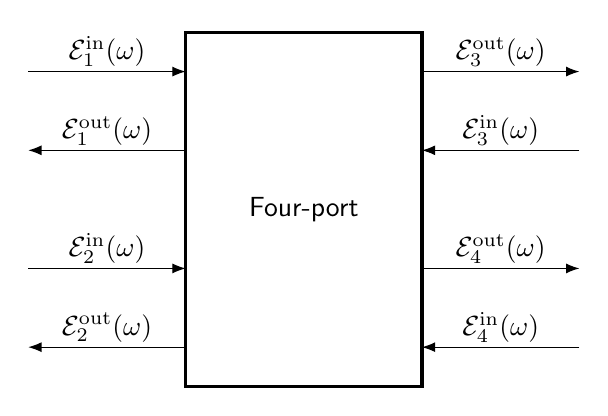
\begin{tikzpicture}[
    	arrow/.style={-Latex},
    ]
        \draw[very thick] (0, 0) rectangle (3, 4.5);
        \node[text width=4cm, align=center] at (1.5, 2.25) {\textsf{Four-port}};

        \draw[arrow] (-2, 4) -- ++(2, 0) node(in1a){};
        \draw[arrow] (in1a) ++(0, -1) node(in1b){} -- ++(-2, 0);
        \draw (in1a) ++(-1, 0.25) node{$\mathcal{E}^{\text{in}}_1(\omega)$};
        \draw (in1b) ++(-1, 0.25) node{$\mathcal{E}^{\text{out}}_1(\omega)$};

        \draw[arrow] (in1b) ++(-2, -1.5) -- ++(2, 0) node(in2a){};
        \draw[arrow] (in2a) ++(0, -1) node(in2b){} -- ++(-2, 0);
        \draw (in2a) ++(-1, 0.25) node{$\mathcal{E}^{\text{in}}_2(\omega)$};
        \draw (in2b) ++(-1, 0.25) node{$\mathcal{E}^{\text{out}}_2(\omega)$};

        \draw[arrow] (in1a) ++(3, 0) node(out1a){} -- ++(2, 0);
        \draw[arrow] (in1b) ++(5, 0) -- ++(-2, 0) node(out1b){};
        \draw (out1a) ++(1, 0.25) node{$\mathcal{E}^{\text{out}}_3(\omega)$};
        \draw (out1b) ++(1, 0.25) node{$\mathcal{E}^{\text{in}}_3(\omega)$};

        \draw[arrow] (in2a) ++(3, 0) node(out2a){} -- ++(2, 0);
        \draw[arrow] (in2b) ++(5, 0) -- ++(-2, 0) node(out2b){};
        \draw (out2a) ++(1, 0.25) node{$\mathcal{E}^{\text{out}}_4(\omega)$};
        \draw (out2b) ++(1, 0.25) node{$\mathcal{E}^{\text{in}}_4(\omega)$};
    \end{tikzpicture}
\end{document}
